\documentclass[twoside]{book}

% Packages required by doxygen
\usepackage{calc}
\usepackage{doxygen}
\usepackage{graphicx}
\usepackage[utf8]{inputenc}
\usepackage{makeidx}
\usepackage{multicol}
\usepackage{multirow}
\usepackage{textcomp}
\usepackage[table]{xcolor}

% Font selection
\usepackage[T1]{fontenc}
\usepackage{mathptmx}
\usepackage[scaled=.90]{helvet}
\usepackage{courier}
\usepackage{amssymb}
\usepackage{sectsty}
\renewcommand{\familydefault}{\sfdefault}
\allsectionsfont{%
  \fontseries{bc}\selectfont%
  \color{darkgray}%
}
\renewcommand{\DoxyLabelFont}{%
  \fontseries{bc}\selectfont%
  \color{darkgray}%
}

% Page & text layout
\usepackage{geometry}
\geometry{%
  a4paper,%
  top=2.5cm,%
  bottom=2.5cm,%
  left=2.5cm,%
  right=2.5cm%
}
\tolerance=750
\hfuzz=15pt
\hbadness=750
\setlength{\emergencystretch}{15pt}
\setlength{\parindent}{0cm}
\setlength{\parskip}{0.2cm}
\makeatletter
\renewcommand{\paragraph}{%
  \@startsection{paragraph}{4}{0ex}{-1.0ex}{1.0ex}{%
    \normalfont\normalsize\bfseries\SS@parafont%
  }%
}
\renewcommand{\subparagraph}{%
  \@startsection{subparagraph}{5}{0ex}{-1.0ex}{1.0ex}{%
    \normalfont\normalsize\bfseries\SS@subparafont%
  }%
}
\makeatother

% Headers & footers
\usepackage{fancyhdr}
\pagestyle{fancyplain}
\fancyhead[LE]{\fancyplain{}{\bfseries\thepage}}
\fancyhead[CE]{\fancyplain{}{}}
\fancyhead[RE]{\fancyplain{}{\bfseries\leftmark}}
\fancyhead[LO]{\fancyplain{}{\bfseries\rightmark}}
\fancyhead[CO]{\fancyplain{}{}}
\fancyhead[RO]{\fancyplain{}{\bfseries\thepage}}
\fancyfoot[LE]{\fancyplain{}{}}
\fancyfoot[CE]{\fancyplain{}{}}
\fancyfoot[RE]{\fancyplain{}{\bfseries\scriptsize Generated on Wed May 27 2015 22\-:27\-:19 for My Project by Doxygen }}
\fancyfoot[LO]{\fancyplain{}{\bfseries\scriptsize Generated on Wed May 27 2015 22\-:27\-:19 for My Project by Doxygen }}
\fancyfoot[CO]{\fancyplain{}{}}
\fancyfoot[RO]{\fancyplain{}{}}
\renewcommand{\footrulewidth}{0.4pt}
\renewcommand{\chaptermark}[1]{%
  \markboth{#1}{}%
}
\renewcommand{\sectionmark}[1]{%
  \markright{\thesection\ #1}%
}

% Indices & bibliography
\usepackage{natbib}
\usepackage[titles]{tocloft}
\setcounter{tocdepth}{3}
\setcounter{secnumdepth}{5}
\makeindex

% Hyperlinks (required, but should be loaded last)
\usepackage{ifpdf}
\ifpdf
  \usepackage[pdftex,pagebackref=true]{hyperref}
\else
  \usepackage[ps2pdf,pagebackref=true]{hyperref}
\fi
\hypersetup{%
  colorlinks=true,%
  linkcolor=blue,%
  citecolor=blue,%
  unicode%
}

% Custom commands
\newcommand{\clearemptydoublepage}{%
  \newpage{\pagestyle{empty}\cleardoublepage}%
}


%===== C O N T E N T S =====

\begin{document}

% Titlepage & ToC
\hypersetup{pageanchor=false}
\pagenumbering{roman}
\begin{titlepage}
\vspace*{7cm}
\begin{center}%
{\Large My Project }\\
\vspace*{1cm}
{\large Generated by Doxygen 1.8.6}\\
\vspace*{0.5cm}
{\small Wed May 27 2015 22:27:19}\\
\end{center}
\end{titlepage}
\clearemptydoublepage
\tableofcontents
\clearemptydoublepage
\pagenumbering{arabic}
\hypersetup{pageanchor=true}

%--- Begin generated contents ---
\chapter{Hierarchical Index}
\section{Class Hierarchy}
This inheritance list is sorted roughly, but not completely, alphabetically\-:\begin{DoxyCompactList}
\item \contentsline{section}{Camera}{\pageref{classCamera}}{}
\item \contentsline{section}{camera}{\pageref{classcamera}}{}
\item \contentsline{section}{C\-G}{\pageref{classCG}}{}
\item \contentsline{section}{Directional\-Light}{\pageref{structDirectionalLight}}{}
\item \contentsline{section}{Gerenciador\-Grafico}{\pageref{classGerenciadorGrafico}}{}
\item \contentsline{section}{Lighting}{\pageref{classLighting}}{}
\item \contentsline{section}{Material}{\pageref{structMaterial}}{}
\item \contentsline{section}{math\-\_\-3d}{\pageref{classmath__3d}}{}
\item \contentsline{section}{Matrix4f}{\pageref{classMatrix4f}}{}
\item \contentsline{section}{Mesh}{\pageref{classMesh}}{}
\item \contentsline{section}{mesh}{\pageref{classmesh}}{}
\item \contentsline{section}{ogldev\-\_\-math\-\_\-3d}{\pageref{classogldev__math__3d}}{}
\item \contentsline{section}{ogldev\-\_\-texture}{\pageref{classogldev__texture}}{}
\item \contentsline{section}{ogldev\-\_\-types}{\pageref{classogldev__types}}{}
\item \contentsline{section}{ogldev\-\_\-util}{\pageref{classogldev__util}}{}
\item \contentsline{section}{Orientation}{\pageref{structOrientation}}{}
\item \contentsline{section}{Pers\-Proj\-Info}{\pageref{structPersProjInfo}}{}
\item \contentsline{section}{Pipeline}{\pageref{classPipeline}}{}
\item \contentsline{section}{pipeline}{\pageref{classpipeline}}{}
\item \contentsline{section}{Quaternion}{\pageref{structQuaternion}}{}
\item \contentsline{section}{shader}{\pageref{classshader}}{}
\item \contentsline{section}{technique}{\pageref{classtechnique}}{}
\item \contentsline{section}{Technique}{\pageref{classTechnique}}{}
\begin{DoxyCompactList}
\item \contentsline{section}{Lighting\-Technique}{\pageref{classLightingTechnique}}{}
\end{DoxyCompactList}
\item \contentsline{section}{Texture}{\pageref{classTexture}}{}
\item \contentsline{section}{vec}{\pageref{classvec}}{}
\item \contentsline{section}{Vector2f}{\pageref{structVector2f}}{}
\item \contentsline{section}{Vector2i}{\pageref{structVector2i}}{}
\item \contentsline{section}{Vector3f}{\pageref{structVector3f}}{}
\item \contentsline{section}{Vector4f}{\pageref{structVector4f}}{}
\item \contentsline{section}{Vertex}{\pageref{structVertex}}{}
\item \contentsline{section}{Vertex2\-D}{\pageref{structVertex2D}}{}
\end{DoxyCompactList}

\chapter{Class Index}
\section{Class List}
Here are the classes, structs, unions and interfaces with brief descriptions\-:\begin{DoxyCompactList}
\item\contentsline{section}{\hyperlink{classCamera}{Camera} }{\pageref{classCamera}}{}
\item\contentsline{section}{\hyperlink{classcamera}{camera} \\*Classe da câmera Classe Destinada a parte de Gerenciamento da câmera da aplicação, contando com movimentação da câmera da cena }{\pageref{classcamera}}{}
\item\contentsline{section}{\hyperlink{classCG}{C\-G} \\*Classe de gerenciamento gráfico Classe Destinada a parte de Gerenciamento Gráfico da aplicação, contando com disponibilização da tela e renderização }{\pageref{classCG}}{}
\item\contentsline{section}{\hyperlink{structDirectionalLight}{Directional\-Light} }{\pageref{structDirectionalLight}}{}
\item\contentsline{section}{\hyperlink{classGerenciadorGrafico}{Gerenciador\-Grafico} }{\pageref{classGerenciadorGrafico}}{}
\item\contentsline{section}{\hyperlink{classLighting}{Lighting} \\*Classe da luminosidade Classe Destinada a parte de Gerenciamento da luminosidade da aplicação, contando com tipo e intensidade da luz }{\pageref{classLighting}}{}
\item\contentsline{section}{\hyperlink{classLightingTechnique}{Lighting\-Technique} }{\pageref{classLightingTechnique}}{}
\item\contentsline{section}{\hyperlink{structMaterial}{Material} }{\pageref{structMaterial}}{}
\item\contentsline{section}{\hyperlink{classmath__3d}{math\-\_\-3d} \\*Classe de cálculos relativos aos objetos Classe Destinada a parte de cálculos dos objetos da cena, contando com cálculo de normalização, rotação, transformação, inversa e outros }{\pageref{classmath__3d}}{}
\item\contentsline{section}{\hyperlink{classMatrix4f}{Matrix4f} }{\pageref{classMatrix4f}}{}
\item\contentsline{section}{\hyperlink{classMesh}{Mesh} }{\pageref{classMesh}}{}
\item\contentsline{section}{\hyperlink{classmesh}{mesh} \\*Classe \hyperlink{classMesh}{Mesh} Classe Destinada a parte de textura, contando com cálculo de delta e imagem da textura }{\pageref{classmesh}}{}
\item\contentsline{section}{\hyperlink{classogldev__math__3d}{ogldev\-\_\-math\-\_\-3d} \\*Classe \hyperlink{classogldev__math__3d}{ogldev\-\_\-math\-\_\-3d} Classe Destinada a parte de cálculos dos objetos da cena }{\pageref{classogldev__math__3d}}{}
\item\contentsline{section}{\hyperlink{classogldev__texture}{ogldev\-\_\-texture} \\*Classe de textura Classe Destinada a parte de Gerenciamento de textura dos objetos da aplicação }{\pageref{classogldev__texture}}{}
\item\contentsline{section}{\hyperlink{classogldev__types}{ogldev\-\_\-types} \\*Classe de tipos }{\pageref{classogldev__types}}{}
\item\contentsline{section}{\hyperlink{classogldev__util}{ogldev\-\_\-util} \\*Classe de utilidades Classe Destinada a utilidades aquém das demais classes ogldev }{\pageref{classogldev__util}}{}
\item\contentsline{section}{\hyperlink{structOrientation}{Orientation} }{\pageref{structOrientation}}{}
\item\contentsline{section}{\hyperlink{structPersProjInfo}{Pers\-Proj\-Info} }{\pageref{structPersProjInfo}}{}
\item\contentsline{section}{\hyperlink{classPipeline}{Pipeline} }{\pageref{classPipeline}}{}
\item\contentsline{section}{\hyperlink{classpipeline}{pipeline} \\*Classe do pipeline da aplicação Classe Destinada ao gerenciamento e utilização do pipeline da G\-P\-U, para transformações }{\pageref{classpipeline}}{}
\item\contentsline{section}{\hyperlink{structQuaternion}{Quaternion} }{\pageref{structQuaternion}}{}
\item\contentsline{section}{\hyperlink{classshader}{shader} \\*Classe do shader da aplicação Classe Destinada ao shader da aplicação }{\pageref{classshader}}{}
\item\contentsline{section}{\hyperlink{classtechnique}{technique} \\*Classe de técnicas da aplicação Classe Destinada ao gerenciamento e utilização do shader da aplicação e os objetos }{\pageref{classtechnique}}{}
\item\contentsline{section}{\hyperlink{classTechnique}{Technique} }{\pageref{classTechnique}}{}
\item\contentsline{section}{\hyperlink{classTexture}{Texture} }{\pageref{classTexture}}{}
\item\contentsline{section}{\hyperlink{classvec}{vec} \\*Classe de estrutura de dados da aplicação Classe Destinada a criação e gerenciamento da estrutura de dados da aplicação }{\pageref{classvec}}{}
\item\contentsline{section}{\hyperlink{structVector2f}{Vector2f} }{\pageref{structVector2f}}{}
\item\contentsline{section}{\hyperlink{structVector2i}{Vector2i} }{\pageref{structVector2i}}{}
\item\contentsline{section}{\hyperlink{structVector3f}{Vector3f} }{\pageref{structVector3f}}{}
\item\contentsline{section}{\hyperlink{structVector4f}{Vector4f} }{\pageref{structVector4f}}{}
\item\contentsline{section}{\hyperlink{structVertex}{Vertex} }{\pageref{structVertex}}{}
\item\contentsline{section}{\hyperlink{structVertex2D}{Vertex2\-D} }{\pageref{structVertex2D}}{}
\end{DoxyCompactList}

\chapter{Class Documentation}
\hypertarget{classCamera}{\section{Camera Class Reference}
\label{classCamera}\index{Camera@{Camera}}
}
\subsection*{Public Member Functions}
\begin{DoxyCompactItemize}
\item 
\hypertarget{classCamera_a21ebfdad71ca67ec496f16b50e013d21}{{\bfseries Camera} (const \hyperlink{structVector3f}{Vector3f} \&Pos, const \hyperlink{structVector3f}{Vector3f} \&Target, const \hyperlink{structVector3f}{Vector3f} \&Up)}\label{classCamera_a21ebfdad71ca67ec496f16b50e013d21}

\item 
\hypertarget{classCamera_a93809e953f183cd95568e2e1a06de2b3}{bool {\bfseries On\-Keyboard} (int Key)}\label{classCamera_a93809e953f183cd95568e2e1a06de2b3}

\item 
\hypertarget{classCamera_aba5837fa7cb0cc4cc421e07cf6566cff}{const \hyperlink{structVector3f}{Vector3f} \& {\bfseries Get\-Pos} () const }\label{classCamera_aba5837fa7cb0cc4cc421e07cf6566cff}

\item 
\hypertarget{classCamera_a601ded4bbaf03c798abf646c21ff64a3}{const \hyperlink{structVector3f}{Vector3f} \& {\bfseries Get\-Target} () const }\label{classCamera_a601ded4bbaf03c798abf646c21ff64a3}

\item 
\hypertarget{classCamera_af4647e8efeeefc8158169b428091015f}{const \hyperlink{structVector3f}{Vector3f} \& {\bfseries Get\-Up} () const }\label{classCamera_af4647e8efeeefc8158169b428091015f}

\end{DoxyCompactItemize}


The documentation for this class was generated from the following files\-:\begin{DoxyCompactItemize}
\item 
camera.\-h\item 
camera.\-cpp\end{DoxyCompactItemize}

\hypertarget{classcamera}{\section{camera Class Reference}
\label{classcamera}\index{camera@{camera}}
}


Classe da câmera Classe Destinada a parte de Gerenciamento da câmera da aplicação, contando com movimentação da câmera da cena.  




{\ttfamily \#include $<$camera.\-h$>$}



\subsection{Detailed Description}
Classe da câmera Classe Destinada a parte de Gerenciamento da câmera da aplicação, contando com movimentação da câmera da cena. 

The documentation for this class was generated from the following file\-:\begin{DoxyCompactItemize}
\item 
camera.\-h\end{DoxyCompactItemize}

\hypertarget{classCG}{\section{C\-G Class Reference}
\label{classCG}\index{C\-G@{C\-G}}
}


Classe de gerenciamento gráfico Classe Destinada a parte de Gerenciamento Gráfico da aplicação, contando com disponibilização da tela e renderização.  




{\ttfamily \#include $<$C\-G.\-h$>$}



\subsection{Detailed Description}
Classe de gerenciamento gráfico Classe Destinada a parte de Gerenciamento Gráfico da aplicação, contando com disponibilização da tela e renderização. 

The documentation for this class was generated from the following file\-:\begin{DoxyCompactItemize}
\item 
C\-G.\-h\end{DoxyCompactItemize}

\hypertarget{structDirectionalLight}{\section{Directional\-Light Struct Reference}
\label{structDirectionalLight}\index{Directional\-Light@{Directional\-Light}}
}
\subsection*{Public Attributes}
\begin{DoxyCompactItemize}
\item 
\hypertarget{structDirectionalLight_a4fd9e75b57df50471d19fe830dd30ef1}{\hyperlink{structVector3f}{Vector3f} {\bfseries Color}}\label{structDirectionalLight_a4fd9e75b57df50471d19fe830dd30ef1}

\item 
\hypertarget{structDirectionalLight_a201a586adf416c65cc017f1549753612}{float {\bfseries Ambient\-Intensity}}\label{structDirectionalLight_a201a586adf416c65cc017f1549753612}

\item 
\hypertarget{structDirectionalLight_a4971d26a6f2f4a4c5b7cee724b9516af}{\hyperlink{structVector3f}{Vector3f} {\bfseries Direction}}\label{structDirectionalLight_a4971d26a6f2f4a4c5b7cee724b9516af}

\item 
\hypertarget{structDirectionalLight_a53f3ba9e4df1a218949483c253693397}{float {\bfseries Diffuse\-Intensity}}\label{structDirectionalLight_a53f3ba9e4df1a218949483c253693397}

\end{DoxyCompactItemize}


The documentation for this struct was generated from the following file\-:\begin{DoxyCompactItemize}
\item 
lighting\-\_\-technique.\-h\end{DoxyCompactItemize}

\hypertarget{classGerenciadorGrafico}{\section{Gerenciador\-Grafico Class Reference}
\label{classGerenciadorGrafico}\index{Gerenciador\-Grafico@{Gerenciador\-Grafico}}
}
\subsection*{Public Member Functions}
\begin{DoxyCompactItemize}
\item 
\hypertarget{classGerenciadorGrafico_a0213dce4e0ea77b2b1b2ee4833f9ef5c}{{\bfseries Gerenciador\-Grafico} (int largura=800, int altura=600)}\label{classGerenciadorGrafico_a0213dce4e0ea77b2b1b2ee4833f9ef5c}

\item 
\hypertarget{classGerenciadorGrafico_a880153d59789958ae68cebe650a6063f}{void {\bfseries iniciar\-G\-L} ()}\label{classGerenciadorGrafico_a880153d59789958ae68cebe650a6063f}

\item 
\hypertarget{classGerenciadorGrafico_a220eb59ca4dfebd111c10e7b6f3e1a65}{int {\bfseries set\-View\-Port} (int, int)}\label{classGerenciadorGrafico_a220eb59ca4dfebd111c10e7b6f3e1a65}

\item 
\hypertarget{classGerenciadorGrafico_aa0b7c377a12fffdbc382dc72c3384c28}{void {\bfseries delay} (int)}\label{classGerenciadorGrafico_aa0b7c377a12fffdbc382dc72c3384c28}

\item 
\hypertarget{classGerenciadorGrafico_a81a942fc91012655361c466d182b296c}{void {\bfseries iniciar\-Render} ()}\label{classGerenciadorGrafico_a81a942fc91012655361c466d182b296c}

\item 
\hypertarget{classGerenciadorGrafico_a542235e066f0653ef86014803fde262a}{void {\bfseries display\-Render} ()}\label{classGerenciadorGrafico_a542235e066f0653ef86014803fde262a}

\end{DoxyCompactItemize}


The documentation for this class was generated from the following files\-:\begin{DoxyCompactItemize}
\item 
C\-G.\-h\item 
C\-G.\-cpp\end{DoxyCompactItemize}

\hypertarget{classLighting}{\section{Lighting Class Reference}
\label{classLighting}\index{Lighting@{Lighting}}
}


Classe da luminosidade Classe Destinada a parte de Gerenciamento da luminosidade da aplicação, contando com tipo e intensidade da luz.  




\subsection{Detailed Description}
Classe da luminosidade Classe Destinada a parte de Gerenciamento da luminosidade da aplicação, contando com tipo e intensidade da luz. 

The documentation for this class was generated from the following file\-:\begin{DoxyCompactItemize}
\item 
lighting\-\_\-technique.\-h\end{DoxyCompactItemize}

\hypertarget{classLightingTechnique}{\section{Lighting\-Technique Class Reference}
\label{classLightingTechnique}\index{Lighting\-Technique@{Lighting\-Technique}}
}
Inheritance diagram for Lighting\-Technique\-:\begin{figure}[H]
\begin{center}
\leavevmode
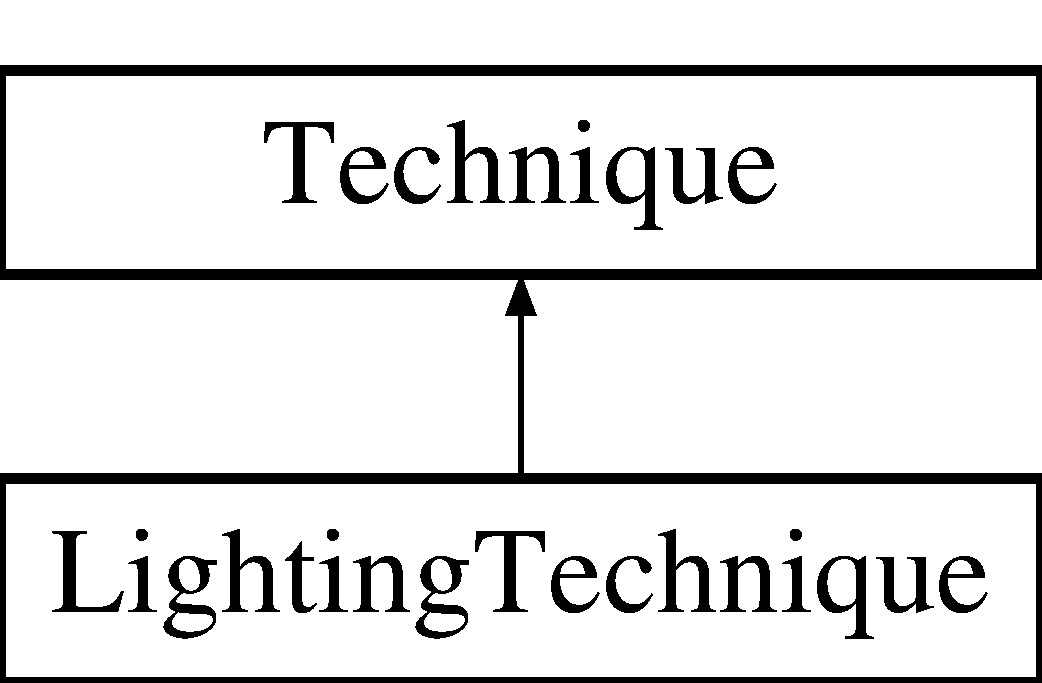
\includegraphics[height=2.000000cm]{classLightingTechnique}
\end{center}
\end{figure}
\subsection*{Public Member Functions}
\begin{DoxyCompactItemize}
\item 
\hypertarget{classLightingTechnique_a0409e6158672177277d756d3e0585c4d}{virtual bool {\bfseries Init} ()}\label{classLightingTechnique_a0409e6158672177277d756d3e0585c4d}

\item 
\hypertarget{classLightingTechnique_a30d9a915fac215d5b86c43bc6285ae30}{void {\bfseries Set\-W\-V\-P} (const \hyperlink{classMatrix4f}{Matrix4f} \&W\-V\-P)}\label{classLightingTechnique_a30d9a915fac215d5b86c43bc6285ae30}

\item 
\hypertarget{classLightingTechnique_a4d8e1b4ae9015f5eef18b808061af22f}{void {\bfseries Set\-Texture\-Unit} (unsigned int Texture\-Unit)}\label{classLightingTechnique_a4d8e1b4ae9015f5eef18b808061af22f}

\item 
\hypertarget{classLightingTechnique_afee3e4439511c07b91aac74d80b25397}{void {\bfseries Set\-Directional\-Light} (const \hyperlink{structDirectionalLight}{Directional\-Light} \&Light)}\label{classLightingTechnique_afee3e4439511c07b91aac74d80b25397}

\end{DoxyCompactItemize}
\subsection*{Additional Inherited Members}


The documentation for this class was generated from the following files\-:\begin{DoxyCompactItemize}
\item 
lighting\-\_\-technique.\-h\item 
lighting\-\_\-technique.\-cpp\end{DoxyCompactItemize}

\hypertarget{structMaterial}{\section{Material Struct Reference}
\label{structMaterial}\index{Material@{Material}}
}
\subsection*{Public Attributes}
\begin{DoxyCompactItemize}
\item 
\hypertarget{structMaterial_acb698dee8dd625a68b470d35c4ce2a52}{int {\bfseries illum}}\label{structMaterial_acb698dee8dd625a68b470d35c4ce2a52}

\item 
\hypertarget{structMaterial_a57ff184aa459ee74ca9f473d1ed60adb}{int {\bfseries image\-I\-D}}\label{structMaterial_a57ff184aa459ee74ca9f473d1ed60adb}

\item 
\hypertarget{structMaterial_ae9ec390fa9b7b370ed70bb95ff6112bf}{int {\bfseries image\-Width}}\label{structMaterial_ae9ec390fa9b7b370ed70bb95ff6112bf}

\item 
\hypertarget{structMaterial_afda76f8ad603920e3f62f3bb17529116}{int {\bfseries image\-Height}}\label{structMaterial_afda76f8ad603920e3f62f3bb17529116}

\item 
\hypertarget{structMaterial_acfda72ce20da4961aa5159ff5be4c6bc}{G\-Luint {\bfseries texture\-I\-D}}\label{structMaterial_acfda72ce20da4961aa5159ff5be4c6bc}

\item 
\hypertarget{structMaterial_afd84d63c7b381ef6f976d4cb685c9f97}{unsigned char $\ast$ {\bfseries image\-Data}}\label{structMaterial_afd84d63c7b381ef6f976d4cb685c9f97}

\item 
\hypertarget{structMaterial_a988570645fdd4363ca975f5bb4e47205}{string {\bfseries name}}\label{structMaterial_a988570645fdd4363ca975f5bb4e47205}

\item 
\hypertarget{structMaterial_a6c689e98f398ee32c623375414334b8c}{string {\bfseries file\-Name}}\label{structMaterial_a6c689e98f398ee32c623375414334b8c}

\item 
\hypertarget{structMaterial_a49335919c5596c4523f71be7f01bdf9d}{float {\bfseries ns}}\label{structMaterial_a49335919c5596c4523f71be7f01bdf9d}

\item 
\hypertarget{structMaterial_a9132d1f6cc468abe6c40659962e06236}{float {\bfseries ni}}\label{structMaterial_a9132d1f6cc468abe6c40659962e06236}

\item 
\hypertarget{structMaterial_a72cb289b8dccb7a08e0b0f7880a92803}{float {\bfseries d}}\label{structMaterial_a72cb289b8dccb7a08e0b0f7880a92803}

\item 
\hypertarget{structMaterial_a1912c2fa001d2df50882076c6b83ef26}{float {\bfseries tr}}\label{structMaterial_a1912c2fa001d2df50882076c6b83ef26}

\item 
\hypertarget{structMaterial_a59d28104e0b4fb52a80136ea2136e583}{float {\bfseries tf} \mbox{[}3\mbox{]}}\label{structMaterial_a59d28104e0b4fb52a80136ea2136e583}

\item 
\hypertarget{structMaterial_ab991cf8e96ff92584c599a0ed16b4c07}{float {\bfseries ka} \mbox{[}3\mbox{]}}\label{structMaterial_ab991cf8e96ff92584c599a0ed16b4c07}

\item 
\hypertarget{structMaterial_a81ac6613710953fa04446cd1c13f8e09}{float {\bfseries kd} \mbox{[}3\mbox{]}}\label{structMaterial_a81ac6613710953fa04446cd1c13f8e09}

\item 
\hypertarget{structMaterial_a0fe4913bbe46ec42aa7320548ad05b24}{float {\bfseries ks} \mbox{[}3\mbox{]}}\label{structMaterial_a0fe4913bbe46ec42aa7320548ad05b24}

\item 
\hypertarget{structMaterial_a492ba6bdcd27816f72640b66d6647b71}{float {\bfseries ke} \mbox{[}3\mbox{]}}\label{structMaterial_a492ba6bdcd27816f72640b66d6647b71}

\end{DoxyCompactItemize}


The documentation for this struct was generated from the following file\-:\begin{DoxyCompactItemize}
\item 
vec.\-h\end{DoxyCompactItemize}

\hypertarget{classmath__3d}{\section{math\-\_\-3d Class Reference}
\label{classmath__3d}\index{math\-\_\-3d@{math\-\_\-3d}}
}


Classe de cálculos relativos aos objetos Classe Destinada a parte de cálculos dos objetos da cena, contando com cálculo de normalização, rotação, transformação, inversa e outros.  




{\ttfamily \#include $<$math\-\_\-3d.\-h$>$}



\subsection{Detailed Description}
Classe de cálculos relativos aos objetos Classe Destinada a parte de cálculos dos objetos da cena, contando com cálculo de normalização, rotação, transformação, inversa e outros. 

The documentation for this class was generated from the following file\-:\begin{DoxyCompactItemize}
\item 
math\-\_\-3d.\-h\end{DoxyCompactItemize}

\hypertarget{classMatrix4f}{\section{Matrix4f Class Reference}
\label{classMatrix4f}\index{Matrix4f@{Matrix4f}}
}
\subsection*{Public Member Functions}
\begin{DoxyCompactItemize}
\item 
\hypertarget{classMatrix4f_a5cedfa71f928157c3ed4516edc72cb9c}{void {\bfseries Init\-Identity} ()}\label{classMatrix4f_a5cedfa71f928157c3ed4516edc72cb9c}

\item 
\hypertarget{classMatrix4f_aaa55b11a3b44065ebaea23750d8f15f2}{\hyperlink{classMatrix4f}{Matrix4f} {\bfseries Transpose} () const }\label{classMatrix4f_aaa55b11a3b44065ebaea23750d8f15f2}

\item 
\hypertarget{classMatrix4f_adbda08a5bee8094658af28bfaa851e1c}{\hyperlink{classMatrix4f}{Matrix4f} {\bfseries operator$\ast$} (const \hyperlink{classMatrix4f}{Matrix4f} \&Right) const }\label{classMatrix4f_adbda08a5bee8094658af28bfaa851e1c}

\item 
\hypertarget{classMatrix4f_ae41adb262631b053ab76c68a36be4c4e}{\hyperlink{structVector4f}{Vector4f} {\bfseries operator$\ast$} (const \hyperlink{structVector4f}{Vector4f} \&v) const }\label{classMatrix4f_ae41adb262631b053ab76c68a36be4c4e}

\item 
\hypertarget{classMatrix4f_ab6bc3cb75cb930b2eed630dda75499d2}{{\bfseries operator const float $\ast$} () const }\label{classMatrix4f_ab6bc3cb75cb930b2eed630dda75499d2}

\item 
\hypertarget{classMatrix4f_a99eef2db139a6334b4d53b5876b364bf}{void {\bfseries Print} () const }\label{classMatrix4f_a99eef2db139a6334b4d53b5876b364bf}

\item 
\hypertarget{classMatrix4f_ab61077c954bd8bcc6f422b2ba9109685}{float {\bfseries Determinant} () const }\label{classMatrix4f_ab61077c954bd8bcc6f422b2ba9109685}

\item 
\hypertarget{classMatrix4f_af1e77173b3f52e2b7a75ca03999d3a4d}{\hyperlink{classMatrix4f}{Matrix4f} \& {\bfseries Inverse} ()}\label{classMatrix4f_af1e77173b3f52e2b7a75ca03999d3a4d}

\item 
\hypertarget{classMatrix4f_aa0552eaded648aa9c77ef72385e79ced}{void {\bfseries Init\-Scale\-Transform} (float Scale\-X, float Scale\-Y, float Scale\-Z)}\label{classMatrix4f_aa0552eaded648aa9c77ef72385e79ced}

\item 
\hypertarget{classMatrix4f_acaba507cb1366b75f353816c8f7c1f81}{void {\bfseries Init\-Rotate\-Transform} (float Rotate\-X, float Rotate\-Y, float Rotate\-Z)}\label{classMatrix4f_acaba507cb1366b75f353816c8f7c1f81}

\item 
\hypertarget{classMatrix4f_aebf4d72c978e7c2c5770da4b2f9b88bb}{void {\bfseries Init\-Translation\-Transform} (float x, float y, float z)}\label{classMatrix4f_aebf4d72c978e7c2c5770da4b2f9b88bb}

\item 
\hypertarget{classMatrix4f_a6e8c636a04e1fc8d81f448cd68a13aea}{void {\bfseries Init\-Camera\-Transform} (const \hyperlink{structVector3f}{Vector3f} \&Target, const \hyperlink{structVector3f}{Vector3f} \&Up)}\label{classMatrix4f_a6e8c636a04e1fc8d81f448cd68a13aea}

\item 
\hypertarget{classMatrix4f_a48064d7cf650e26623cf5371e2ef1b8b}{void {\bfseries Init\-Pers\-Proj\-Transform} (const \hyperlink{structPersProjInfo}{Pers\-Proj\-Info} \&p)}\label{classMatrix4f_a48064d7cf650e26623cf5371e2ef1b8b}

\item 
\hypertarget{classMatrix4f_adecdcb191c856fb8e265a9496e9e1ad2}{{\bfseries Matrix4f} (const ai\-Matrix4x4 \&Assimp\-Matrix)}\label{classMatrix4f_adecdcb191c856fb8e265a9496e9e1ad2}

\item 
\hypertarget{classMatrix4f_a30bb126218b822b00e3365e2a9a55e42}{{\bfseries Matrix4f} (const ai\-Matrix3x3 \&Assimp\-Matrix)}\label{classMatrix4f_a30bb126218b822b00e3365e2a9a55e42}

\item 
\hypertarget{classMatrix4f_a46a6fc0c402055b8832818d66f61bc14}{{\bfseries Matrix4f} (float a00, float a01, float a02, float a03, float a10, float a11, float a12, float a13, float a20, float a21, float a22, float a23, float a30, float a31, float a32, float a33)}\label{classMatrix4f_a46a6fc0c402055b8832818d66f61bc14}

\item 
\hypertarget{classMatrix4f_a7df3ebb63a5ed13b15a31d2e6b507a7e}{void {\bfseries Set\-Zero} ()}\label{classMatrix4f_a7df3ebb63a5ed13b15a31d2e6b507a7e}

\item 
\hypertarget{classMatrix4f_aaa55b11a3b44065ebaea23750d8f15f2}{\hyperlink{classMatrix4f}{Matrix4f} {\bfseries Transpose} () const }\label{classMatrix4f_aaa55b11a3b44065ebaea23750d8f15f2}

\item 
\hypertarget{classMatrix4f_a5cedfa71f928157c3ed4516edc72cb9c}{void {\bfseries Init\-Identity} ()}\label{classMatrix4f_a5cedfa71f928157c3ed4516edc72cb9c}

\item 
\hypertarget{classMatrix4f_adbda08a5bee8094658af28bfaa851e1c}{\hyperlink{classMatrix4f}{Matrix4f} {\bfseries operator$\ast$} (const \hyperlink{classMatrix4f}{Matrix4f} \&Right) const }\label{classMatrix4f_adbda08a5bee8094658af28bfaa851e1c}

\item 
\hypertarget{classMatrix4f_ae41adb262631b053ab76c68a36be4c4e}{\hyperlink{structVector4f}{Vector4f} {\bfseries operator$\ast$} (const \hyperlink{structVector4f}{Vector4f} \&v) const }\label{classMatrix4f_ae41adb262631b053ab76c68a36be4c4e}

\item 
\hypertarget{classMatrix4f_ab6bc3cb75cb930b2eed630dda75499d2}{{\bfseries operator const float $\ast$} () const }\label{classMatrix4f_ab6bc3cb75cb930b2eed630dda75499d2}

\item 
\hypertarget{classMatrix4f_a99eef2db139a6334b4d53b5876b364bf}{void {\bfseries Print} () const }\label{classMatrix4f_a99eef2db139a6334b4d53b5876b364bf}

\item 
\hypertarget{classMatrix4f_ab61077c954bd8bcc6f422b2ba9109685}{float {\bfseries Determinant} () const }\label{classMatrix4f_ab61077c954bd8bcc6f422b2ba9109685}

\item 
\hypertarget{classMatrix4f_a565187a44d253c52b86037855ef84106}{\hyperlink{classMatrix4f}{Matrix4f} \& {\bfseries Inverse} ()}\label{classMatrix4f_a565187a44d253c52b86037855ef84106}

\item 
\hypertarget{classMatrix4f_aa0552eaded648aa9c77ef72385e79ced}{void {\bfseries Init\-Scale\-Transform} (float Scale\-X, float Scale\-Y, float Scale\-Z)}\label{classMatrix4f_aa0552eaded648aa9c77ef72385e79ced}

\item 
\hypertarget{classMatrix4f_acaba507cb1366b75f353816c8f7c1f81}{void {\bfseries Init\-Rotate\-Transform} (float Rotate\-X, float Rotate\-Y, float Rotate\-Z)}\label{classMatrix4f_acaba507cb1366b75f353816c8f7c1f81}

\item 
\hypertarget{classMatrix4f_aebf4d72c978e7c2c5770da4b2f9b88bb}{void {\bfseries Init\-Translation\-Transform} (float x, float y, float z)}\label{classMatrix4f_aebf4d72c978e7c2c5770da4b2f9b88bb}

\item 
\hypertarget{classMatrix4f_a6e8c636a04e1fc8d81f448cd68a13aea}{void {\bfseries Init\-Camera\-Transform} (const \hyperlink{structVector3f}{Vector3f} \&Target, const \hyperlink{structVector3f}{Vector3f} \&Up)}\label{classMatrix4f_a6e8c636a04e1fc8d81f448cd68a13aea}

\item 
\hypertarget{classMatrix4f_a48064d7cf650e26623cf5371e2ef1b8b}{void {\bfseries Init\-Pers\-Proj\-Transform} (const \hyperlink{structPersProjInfo}{Pers\-Proj\-Info} \&p)}\label{classMatrix4f_a48064d7cf650e26623cf5371e2ef1b8b}

\end{DoxyCompactItemize}
\subsection*{Public Attributes}
\begin{DoxyCompactItemize}
\item 
\hypertarget{classMatrix4f_a51f2ef7cfcd591b03bc78c3a958dfd51}{float {\bfseries m} \mbox{[}4\mbox{]}\mbox{[}4\mbox{]}}\label{classMatrix4f_a51f2ef7cfcd591b03bc78c3a958dfd51}

\end{DoxyCompactItemize}


The documentation for this class was generated from the following files\-:\begin{DoxyCompactItemize}
\item 
math\-\_\-3d.\-h\item 
ogldev\-\_\-math\-\_\-3d.\-h\item 
math\-\_\-3d.\-cpp\end{DoxyCompactItemize}

\hypertarget{classMesh}{\section{Mesh Class Reference}
\label{classMesh}\index{Mesh@{Mesh}}
}
\subsection*{Public Member Functions}
\begin{DoxyCompactItemize}
\item 
\hypertarget{classMesh_ae393146539bdb23d6614501c9618357a}{void {\bfseries carregar\-Arquivo} (string nome\-Arquivo)}\label{classMesh_ae393146539bdb23d6614501c9618357a}

\item 
\hypertarget{classMesh_a3a90a7b3e97fac3718fe815826232263}{void {\bfseries redimensionar} ()}\label{classMesh_a3a90a7b3e97fac3718fe815826232263}

\item 
\hypertarget{classMesh_a7bff6f85614fb7d4ef36d0524c07b281}{void {\bfseries normalizar} ()}\label{classMesh_a7bff6f85614fb7d4ef36d0524c07b281}

\item 
\hypertarget{classMesh_aba7fd1e9dddfc8ded653caebb8ac51c3}{void {\bfseries transladar} ()}\label{classMesh_aba7fd1e9dddfc8ded653caebb8ac51c3}

\item 
\hypertarget{classMesh_abdff0e07055abb34f148fbe3844a7dc6}{vector$<$ \hyperlink{structVertex}{Vertex} $>$ {\bfseries get\-Vertex} ()}\label{classMesh_abdff0e07055abb34f148fbe3844a7dc6}

\item 
\hypertarget{classMesh_a1c64e3b7149df6dbb7a260b02e1a6abe}{vector$<$ unsigned int $>$ {\bfseries get\-Indice} ()}\label{classMesh_a1c64e3b7149df6dbb7a260b02e1a6abe}

\end{DoxyCompactItemize}


The documentation for this class was generated from the following files\-:\begin{DoxyCompactItemize}
\item 
mesh.\-h\item 
mesh.\-cpp\end{DoxyCompactItemize}

\hypertarget{classmesh}{\section{mesh Class Reference}
\label{classmesh}\index{mesh@{mesh}}
}


Classe \hyperlink{classMesh}{Mesh} Classe Destinada a parte de textura, contando com cálculo de delta e imagem da textura.  




{\ttfamily \#include $<$mesh.\-h$>$}



\subsection{Detailed Description}
Classe \hyperlink{classMesh}{Mesh} Classe Destinada a parte de textura, contando com cálculo de delta e imagem da textura. 

The documentation for this class was generated from the following file\-:\begin{DoxyCompactItemize}
\item 
mesh.\-h\end{DoxyCompactItemize}

\hypertarget{classogldev__math__3d}{\section{ogldev\-\_\-math\-\_\-3d Class Reference}
\label{classogldev__math__3d}\index{ogldev\-\_\-math\-\_\-3d@{ogldev\-\_\-math\-\_\-3d}}
}


Classe \hyperlink{classogldev__math__3d}{ogldev\-\_\-math\-\_\-3d} Classe Destinada a parte de cálculos dos objetos da cena.  




{\ttfamily \#include $<$ogldev\-\_\-math\-\_\-3d.\-h$>$}



\subsection{Detailed Description}
Classe \hyperlink{classogldev__math__3d}{ogldev\-\_\-math\-\_\-3d} Classe Destinada a parte de cálculos dos objetos da cena. 

The documentation for this class was generated from the following file\-:\begin{DoxyCompactItemize}
\item 
ogldev\-\_\-math\-\_\-3d.\-h\end{DoxyCompactItemize}

\hypertarget{classogldev__texture}{\section{ogldev\-\_\-texture Class Reference}
\label{classogldev__texture}\index{ogldev\-\_\-texture@{ogldev\-\_\-texture}}
}


Classe de textura Classe Destinada a parte de Gerenciamento de textura dos objetos da aplicação.  




{\ttfamily \#include $<$ogldev\-\_\-texture.\-h$>$}



\subsection{Detailed Description}
Classe de textura Classe Destinada a parte de Gerenciamento de textura dos objetos da aplicação. 

The documentation for this class was generated from the following file\-:\begin{DoxyCompactItemize}
\item 
ogldev\-\_\-texture.\-h\end{DoxyCompactItemize}

\hypertarget{classogldev__types}{\section{ogldev\-\_\-types Class Reference}
\label{classogldev__types}\index{ogldev\-\_\-types@{ogldev\-\_\-types}}
}


Classe de tipos.  




{\ttfamily \#include $<$ogldev\-\_\-types.\-h$>$}



\subsection{Detailed Description}
Classe de tipos. 

Classe Destinada a instância de tipos utilizados na aplicação. 

The documentation for this class was generated from the following file\-:\begin{DoxyCompactItemize}
\item 
ogldev\-\_\-types.\-h\end{DoxyCompactItemize}

\hypertarget{classogldev__util}{\section{ogldev\-\_\-util Class Reference}
\label{classogldev__util}\index{ogldev\-\_\-util@{ogldev\-\_\-util}}
}


Classe de utilidades Classe Destinada a utilidades aquém das demais classes ogldev.  




{\ttfamily \#include $<$ogldev\-\_\-util.\-h$>$}



\subsection{Detailed Description}
Classe de utilidades Classe Destinada a utilidades aquém das demais classes ogldev. 

The documentation for this class was generated from the following file\-:\begin{DoxyCompactItemize}
\item 
ogldev\-\_\-util.\-h\end{DoxyCompactItemize}

\hypertarget{structOrientation}{\section{Orientation Struct Reference}
\label{structOrientation}\index{Orientation@{Orientation}}
}
\subsection*{Public Attributes}
\begin{DoxyCompactItemize}
\item 
\hypertarget{structOrientation_aed80d57793a4f51143ea78bc3d247917}{\hyperlink{structVector3f}{Vector3f} {\bfseries m\-\_\-scale}}\label{structOrientation_aed80d57793a4f51143ea78bc3d247917}

\item 
\hypertarget{structOrientation_a9fec232d2c389810a5a992a7d799bf75}{\hyperlink{structVector3f}{Vector3f} {\bfseries m\-\_\-rotation}}\label{structOrientation_a9fec232d2c389810a5a992a7d799bf75}

\item 
\hypertarget{structOrientation_a80cbfad8ad066d273e7b64b7b6b24783}{\hyperlink{structVector3f}{Vector3f} {\bfseries m\-\_\-pos}}\label{structOrientation_a80cbfad8ad066d273e7b64b7b6b24783}

\end{DoxyCompactItemize}


The documentation for this struct was generated from the following file\-:\begin{DoxyCompactItemize}
\item 
pipeline.\-h\end{DoxyCompactItemize}

\hypertarget{structPersProjInfo}{\section{Pers\-Proj\-Info Struct Reference}
\label{structPersProjInfo}\index{Pers\-Proj\-Info@{Pers\-Proj\-Info}}
}
\subsection*{Public Attributes}
\begin{DoxyCompactItemize}
\item 
\hypertarget{structPersProjInfo_ad730c82443fa16104cda3b9d3fa50710}{float {\bfseries F\-O\-V}}\label{structPersProjInfo_ad730c82443fa16104cda3b9d3fa50710}

\item 
\hypertarget{structPersProjInfo_aa9513ab993e3ecbce36954e487995150}{float {\bfseries Width}}\label{structPersProjInfo_aa9513ab993e3ecbce36954e487995150}

\item 
\hypertarget{structPersProjInfo_aef78e4b62ec21fda782cd0d88cdbbdb7}{float {\bfseries Height}}\label{structPersProjInfo_aef78e4b62ec21fda782cd0d88cdbbdb7}

\item 
\hypertarget{structPersProjInfo_a3af7af16a3f33e3de6fe4db6d5413094}{float {\bfseries z\-Near}}\label{structPersProjInfo_a3af7af16a3f33e3de6fe4db6d5413094}

\item 
\hypertarget{structPersProjInfo_abfcb3315b5516ec433acf16ac7e28998}{float {\bfseries z\-Far}}\label{structPersProjInfo_abfcb3315b5516ec433acf16ac7e28998}

\end{DoxyCompactItemize}


The documentation for this struct was generated from the following files\-:\begin{DoxyCompactItemize}
\item 
math\-\_\-3d.\-h\item 
ogldev\-\_\-math\-\_\-3d.\-h\end{DoxyCompactItemize}

\hypertarget{classPipeline}{\section{Pipeline Class Reference}
\label{classPipeline}\index{Pipeline@{Pipeline}}
}
\subsection*{Public Member Functions}
\begin{DoxyCompactItemize}
\item 
\hypertarget{classPipeline_a387e21872c562a1281555f785176c702}{void {\bfseries Scale} (float s)}\label{classPipeline_a387e21872c562a1281555f785176c702}

\item 
\hypertarget{classPipeline_aa6639e2fe18c7edf3be890bed44bdbff}{void {\bfseries Scale} (const \hyperlink{structVector3f}{Vector3f} \&scale)}\label{classPipeline_aa6639e2fe18c7edf3be890bed44bdbff}

\item 
\hypertarget{classPipeline_aa60c3e22cce9d0368d3339d41996f328}{void {\bfseries Scale} (float Scale\-X, float Scale\-Y, float Scale\-Z)}\label{classPipeline_aa60c3e22cce9d0368d3339d41996f328}

\item 
\hypertarget{classPipeline_ac23d6a9d58cb5b3c56e536359a547f5c}{void {\bfseries World\-Pos} (float x, float y, float z)}\label{classPipeline_ac23d6a9d58cb5b3c56e536359a547f5c}

\item 
\hypertarget{classPipeline_a43ed451f986e4e2fb58360a787178dcb}{void {\bfseries World\-Pos} (const \hyperlink{structVector3f}{Vector3f} \&Pos)}\label{classPipeline_a43ed451f986e4e2fb58360a787178dcb}

\item 
\hypertarget{classPipeline_abc888ac10c51be6dbb0f1b6f8b3c4def}{void {\bfseries Rotate} (float Rotate\-X, float Rotate\-Y, float Rotate\-Z)}\label{classPipeline_abc888ac10c51be6dbb0f1b6f8b3c4def}

\item 
\hypertarget{classPipeline_a0f769bee11ed237587e381b8ef1d53d0}{void {\bfseries Rotate} (const \hyperlink{structVector3f}{Vector3f} \&r)}\label{classPipeline_a0f769bee11ed237587e381b8ef1d53d0}

\item 
\hypertarget{classPipeline_a01e87cbcd48fd0c7ac81f0701aeedb1d}{void {\bfseries Set\-Perspective\-Proj} (const \hyperlink{structPersProjInfo}{Pers\-Proj\-Info} \&p)}\label{classPipeline_a01e87cbcd48fd0c7ac81f0701aeedb1d}

\item 
\hypertarget{classPipeline_a9ec3b9c602bafe01ebb33734e8c174bf}{void {\bfseries Set\-Camera} (const \hyperlink{structVector3f}{Vector3f} \&Pos, const \hyperlink{structVector3f}{Vector3f} \&Target, const \hyperlink{structVector3f}{Vector3f} \&Up)}\label{classPipeline_a9ec3b9c602bafe01ebb33734e8c174bf}

\item 
\hypertarget{classPipeline_a7d339b813f78712a916635dc5b5602e5}{void {\bfseries Set\-Camera} (const \hyperlink{classCamera}{Camera} \&\hyperlink{classcamera}{camera})}\label{classPipeline_a7d339b813f78712a916635dc5b5602e5}

\item 
\hypertarget{classPipeline_a98c822f206c02ae3b2e521dd7381bba1}{void {\bfseries Orient} (const \hyperlink{structOrientation}{Orientation} \&o)}\label{classPipeline_a98c822f206c02ae3b2e521dd7381bba1}

\item 
\hypertarget{classPipeline_a31c4a3caff1e2324a1b0e392ad6b71e4}{const \hyperlink{classMatrix4f}{Matrix4f} \& {\bfseries Get\-W\-P\-Trans} ()}\label{classPipeline_a31c4a3caff1e2324a1b0e392ad6b71e4}

\item 
\hypertarget{classPipeline_ac2a974181aeb54efb291ff223fa3aca5}{const \hyperlink{classMatrix4f}{Matrix4f} \& {\bfseries Get\-W\-V\-Trans} ()}\label{classPipeline_ac2a974181aeb54efb291ff223fa3aca5}

\item 
\hypertarget{classPipeline_a3ffc1aec881ee9f08b6cb120185ee0d0}{const \hyperlink{classMatrix4f}{Matrix4f} \& {\bfseries Get\-V\-P\-Trans} ()}\label{classPipeline_a3ffc1aec881ee9f08b6cb120185ee0d0}

\item 
\hypertarget{classPipeline_a20ae073cd6e65969aee42689dd8cc6b6}{const \hyperlink{classMatrix4f}{Matrix4f} \& {\bfseries Get\-W\-V\-P\-Trans} ()}\label{classPipeline_a20ae073cd6e65969aee42689dd8cc6b6}

\item 
\hypertarget{classPipeline_ac072cb72c79c3a47d306e405b3a248de}{const \hyperlink{classMatrix4f}{Matrix4f} \& {\bfseries Get\-World\-Trans} ()}\label{classPipeline_ac072cb72c79c3a47d306e405b3a248de}

\item 
\hypertarget{classPipeline_af2c83d780f08fbe7135914490a16526f}{const \hyperlink{classMatrix4f}{Matrix4f} \& {\bfseries Get\-View\-Trans} ()}\label{classPipeline_af2c83d780f08fbe7135914490a16526f}

\end{DoxyCompactItemize}


The documentation for this class was generated from the following files\-:\begin{DoxyCompactItemize}
\item 
pipeline.\-h\item 
pipeline.\-cpp\end{DoxyCompactItemize}

\hypertarget{classpipeline}{\section{pipeline Class Reference}
\label{classpipeline}\index{pipeline@{pipeline}}
}


Classe do pipeline da aplicação Classe Destinada ao gerenciamento e utilização do pipeline da G\-P\-U, para transformações.  




{\ttfamily \#include $<$pipeline.\-h$>$}



\subsection{Detailed Description}
Classe do pipeline da aplicação Classe Destinada ao gerenciamento e utilização do pipeline da G\-P\-U, para transformações. 

The documentation for this class was generated from the following file\-:\begin{DoxyCompactItemize}
\item 
pipeline.\-h\end{DoxyCompactItemize}

\hypertarget{structQuaternion}{\section{Quaternion Struct Reference}
\label{structQuaternion}\index{Quaternion@{Quaternion}}
}
\subsection*{Public Member Functions}
\begin{DoxyCompactItemize}
\item 
\hypertarget{structQuaternion_af17f4f2abafce070ff473979f18954e1}{{\bfseries Quaternion} (float \-\_\-x, float \-\_\-y, float \-\_\-z, float \-\_\-w)}\label{structQuaternion_af17f4f2abafce070ff473979f18954e1}

\item 
\hypertarget{structQuaternion_a5c08e0c7533e0c1a526a7401f4754910}{void {\bfseries Normalize} ()}\label{structQuaternion_a5c08e0c7533e0c1a526a7401f4754910}

\item 
\hypertarget{structQuaternion_a204460c32aa96a444929934af3910389}{\hyperlink{structQuaternion}{Quaternion} {\bfseries Conjugate} ()}\label{structQuaternion_a204460c32aa96a444929934af3910389}

\item 
\hypertarget{structQuaternion_af17f4f2abafce070ff473979f18954e1}{{\bfseries Quaternion} (float \-\_\-x, float \-\_\-y, float \-\_\-z, float \-\_\-w)}\label{structQuaternion_af17f4f2abafce070ff473979f18954e1}

\item 
\hypertarget{structQuaternion_a5c08e0c7533e0c1a526a7401f4754910}{void {\bfseries Normalize} ()}\label{structQuaternion_a5c08e0c7533e0c1a526a7401f4754910}

\item 
\hypertarget{structQuaternion_a204460c32aa96a444929934af3910389}{\hyperlink{structQuaternion}{Quaternion} {\bfseries Conjugate} ()}\label{structQuaternion_a204460c32aa96a444929934af3910389}

\end{DoxyCompactItemize}
\subsection*{Public Attributes}
\begin{DoxyCompactItemize}
\item 
\hypertarget{structQuaternion_a8b80f191a3155cc0158d2b4f4d50b2cb}{float {\bfseries x}}\label{structQuaternion_a8b80f191a3155cc0158d2b4f4d50b2cb}

\item 
\hypertarget{structQuaternion_a3bd3f270462944423611f44e19d2511b}{float {\bfseries y}}\label{structQuaternion_a3bd3f270462944423611f44e19d2511b}

\item 
\hypertarget{structQuaternion_a625cb732d8ff3083e7852b86b736ab29}{float {\bfseries z}}\label{structQuaternion_a625cb732d8ff3083e7852b86b736ab29}

\item 
\hypertarget{structQuaternion_aa44a65ab99e36f6ab8771030eed8a7ad}{float {\bfseries w}}\label{structQuaternion_aa44a65ab99e36f6ab8771030eed8a7ad}

\end{DoxyCompactItemize}


The documentation for this struct was generated from the following files\-:\begin{DoxyCompactItemize}
\item 
math\-\_\-3d.\-h\item 
ogldev\-\_\-math\-\_\-3d.\-h\item 
math\-\_\-3d.\-cpp\end{DoxyCompactItemize}

\hypertarget{classshader}{\section{shader Class Reference}
\label{classshader}\index{shader@{shader}}
}


Classe do shader da aplicação Classe Destinada ao shader da aplicação.  




\subsection{Detailed Description}
Classe do shader da aplicação Classe Destinada ao shader da aplicação. 

The documentation for this class was generated from the following file\-:\begin{DoxyCompactItemize}
\item 
shader.\-cpp\end{DoxyCompactItemize}

\hypertarget{classtechnique}{\section{technique Class Reference}
\label{classtechnique}\index{technique@{technique}}
}


Classe de técnicas da aplicação Classe Destinada ao gerenciamento e utilização do shader da aplicação e os objetos.  




{\ttfamily \#include $<$technique.\-h$>$}



\subsection{Detailed Description}
Classe de técnicas da aplicação Classe Destinada ao gerenciamento e utilização do shader da aplicação e os objetos. 

The documentation for this class was generated from the following file\-:\begin{DoxyCompactItemize}
\item 
technique.\-h\end{DoxyCompactItemize}

\hypertarget{classTechnique}{\section{Technique Class Reference}
\label{classTechnique}\index{Technique@{Technique}}
}
Inheritance diagram for Technique\-:\begin{figure}[H]
\begin{center}
\leavevmode
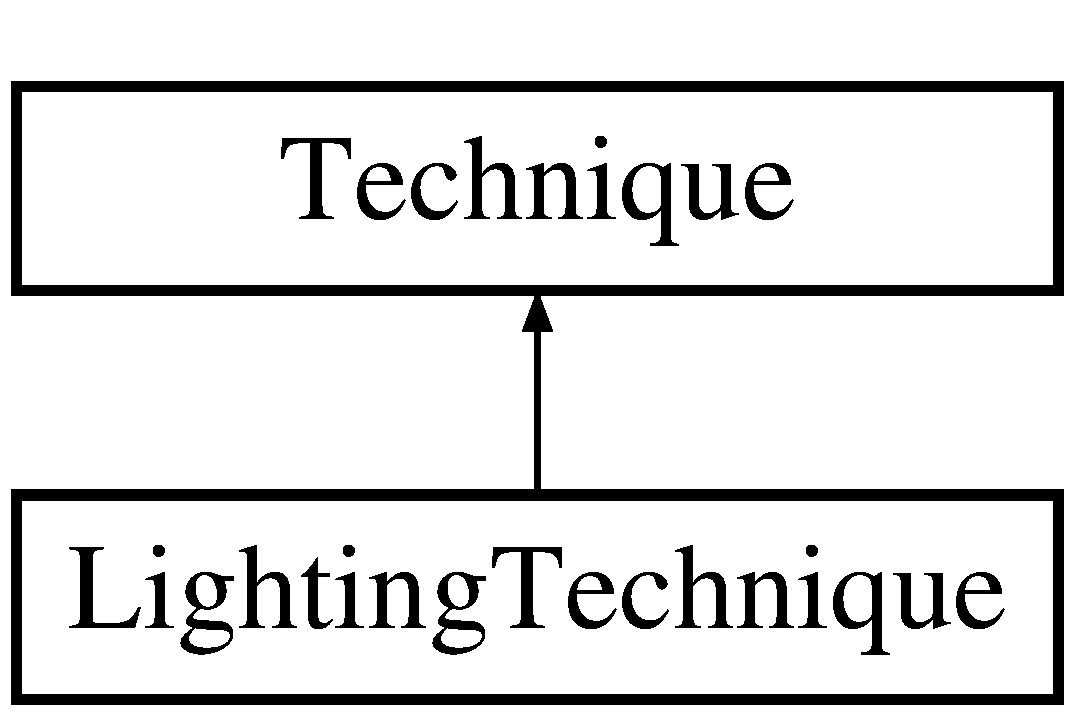
\includegraphics[height=2.000000cm]{classTechnique}
\end{center}
\end{figure}
\subsection*{Public Member Functions}
\begin{DoxyCompactItemize}
\item 
\hypertarget{classTechnique_a3069d5cf658e38c33bfe58da0a5f8da9}{virtual bool {\bfseries Init} ()}\label{classTechnique_a3069d5cf658e38c33bfe58da0a5f8da9}

\item 
\hypertarget{classTechnique_a81be1d1aa3e0796cbd9bbca8f4e134e2}{void {\bfseries Enable} ()}\label{classTechnique_a81be1d1aa3e0796cbd9bbca8f4e134e2}

\end{DoxyCompactItemize}
\subsection*{Protected Member Functions}
\begin{DoxyCompactItemize}
\item 
\hypertarget{classTechnique_acf9cabc2c61a760c5a82b8414b04a5fc}{bool {\bfseries Add\-Shader} (G\-Lenum Shader\-Type, const char $\ast$p\-Filename)}\label{classTechnique_acf9cabc2c61a760c5a82b8414b04a5fc}

\item 
\hypertarget{classTechnique_a19512f7930347cb9132168da0c929a9d}{bool {\bfseries Finalize} ()}\label{classTechnique_a19512f7930347cb9132168da0c929a9d}

\item 
\hypertarget{classTechnique_a618a81179129728e48865511345e8b59}{G\-Lint {\bfseries Get\-Uniform\-Location} (const char $\ast$p\-Uniform\-Name)}\label{classTechnique_a618a81179129728e48865511345e8b59}

\item 
\hypertarget{classTechnique_afb06b0b9660c054f1d6ccdb0312d5ab4}{G\-Lint {\bfseries Get\-Program\-Param} (G\-Lint param)}\label{classTechnique_afb06b0b9660c054f1d6ccdb0312d5ab4}

\end{DoxyCompactItemize}
\subsection*{Protected Attributes}
\begin{DoxyCompactItemize}
\item 
\hypertarget{classTechnique_aa8c85adee2e88ac33e334986059a2ee3}{G\-Luint {\bfseries m\-\_\-shader\-Prog}}\label{classTechnique_aa8c85adee2e88ac33e334986059a2ee3}

\end{DoxyCompactItemize}


The documentation for this class was generated from the following files\-:\begin{DoxyCompactItemize}
\item 
technique.\-h\item 
technique.\-cpp\end{DoxyCompactItemize}

\hypertarget{classTexture}{\section{Texture Class Reference}
\label{classTexture}\index{Texture@{Texture}}
}
\subsection*{Public Member Functions}
\begin{DoxyCompactItemize}
\item 
\hypertarget{classTexture_ab4694b9f76d6e348a844065481a89aa1}{{\bfseries Texture} (G\-Lenum Texture\-Target, const std\-::string \&File\-Name)}\label{classTexture_ab4694b9f76d6e348a844065481a89aa1}

\item 
\hypertarget{classTexture_a4ccaf8f0017dd26ccd824fc2e24c9a27}{bool {\bfseries Load} ()}\label{classTexture_a4ccaf8f0017dd26ccd824fc2e24c9a27}

\item 
\hypertarget{classTexture_afac0ee53fc89f153418d6cfa6f575fbe}{void {\bfseries Bind} (G\-Lenum Texture\-Unit)}\label{classTexture_afac0ee53fc89f153418d6cfa6f575fbe}

\end{DoxyCompactItemize}


The documentation for this class was generated from the following files\-:\begin{DoxyCompactItemize}
\item 
ogldev\-\_\-texture.\-h\item 
ogldev\-\_\-texture.\-cpp\end{DoxyCompactItemize}

\hypertarget{classvec}{\section{vec Class Reference}
\label{classvec}\index{vec@{vec}}
}


Classe de estrutura de dados da aplicação Classe Destinada a criação e gerenciamento da estrutura de dados da aplicação.  




{\ttfamily \#include $<$vec.\-h$>$}



\subsection{Detailed Description}
Classe de estrutura de dados da aplicação Classe Destinada a criação e gerenciamento da estrutura de dados da aplicação. 

The documentation for this class was generated from the following file\-:\begin{DoxyCompactItemize}
\item 
vec.\-h\end{DoxyCompactItemize}

\hypertarget{structVector2f}{\section{Vector2f Struct Reference}
\label{structVector2f}\index{Vector2f@{Vector2f}}
}
\subsection*{Public Member Functions}
\begin{DoxyCompactItemize}
\item 
\hypertarget{structVector2f_a4d82d9240b5de271e5e45c16e8de561e}{{\bfseries Vector2f} (float \-\_\-x, float \-\_\-y)}\label{structVector2f_a4d82d9240b5de271e5e45c16e8de561e}

\item 
\hypertarget{structVector2f_a4d82d9240b5de271e5e45c16e8de561e}{{\bfseries Vector2f} (float \-\_\-x, float \-\_\-y)}\label{structVector2f_a4d82d9240b5de271e5e45c16e8de561e}

\end{DoxyCompactItemize}
\subsection*{Public Attributes}
\begin{DoxyCompactItemize}
\item 
\hypertarget{structVector2f_add58d2378e3a3abdb76cf0ac51c9acfc}{float {\bfseries x}}\label{structVector2f_add58d2378e3a3abdb76cf0ac51c9acfc}

\item 
\hypertarget{structVector2f_a14874a72597fd358b15f8ba34b999c4d}{float {\bfseries y}}\label{structVector2f_a14874a72597fd358b15f8ba34b999c4d}

\end{DoxyCompactItemize}


The documentation for this struct was generated from the following files\-:\begin{DoxyCompactItemize}
\item 
math\-\_\-3d.\-h\item 
ogldev\-\_\-math\-\_\-3d.\-h\end{DoxyCompactItemize}

\hypertarget{structVector2i}{\section{Vector2i Struct Reference}
\label{structVector2i}\index{Vector2i@{Vector2i}}
}
\subsection*{Public Attributes}
\begin{DoxyCompactItemize}
\item 
\hypertarget{structVector2i_ad63e78f71457439cc910f38cfa019b4e}{int {\bfseries x}}\label{structVector2i_ad63e78f71457439cc910f38cfa019b4e}

\item 
\hypertarget{structVector2i_a9a3ca58ba0f5d84bf305ddca107780d8}{int {\bfseries y}}\label{structVector2i_a9a3ca58ba0f5d84bf305ddca107780d8}

\end{DoxyCompactItemize}


The documentation for this struct was generated from the following files\-:\begin{DoxyCompactItemize}
\item 
math\-\_\-3d.\-h\item 
ogldev\-\_\-math\-\_\-3d.\-h\end{DoxyCompactItemize}

\hypertarget{structVector3f}{\section{Vector3f Struct Reference}
\label{structVector3f}\index{Vector3f@{Vector3f}}
}
\subsection*{Public Member Functions}
\begin{DoxyCompactItemize}
\item 
\hypertarget{structVector3f_ac2caf1fd41076826fe50b3a527ef90db}{{\bfseries Vector3f} (float \-\_\-x, float \-\_\-y, float \-\_\-z)}\label{structVector3f_ac2caf1fd41076826fe50b3a527ef90db}

\end{DoxyCompactItemize}
\subsection*{Public Attributes}
\begin{DoxyCompactItemize}
\item 
\hypertarget{structVector3f_a4aca0751716b7099b397e8c63b16bfcf}{float {\bfseries x}}\label{structVector3f_a4aca0751716b7099b397e8c63b16bfcf}

\item 
\hypertarget{structVector3f_a8a602e2ee75126feb520c2aa27e7eff5}{float {\bfseries y}}\label{structVector3f_a8a602e2ee75126feb520c2aa27e7eff5}

\item 
\hypertarget{structVector3f_a470cff51eb6463672be518f5af4e26db}{float {\bfseries z}}\label{structVector3f_a470cff51eb6463672be518f5af4e26db}

\end{DoxyCompactItemize}


The documentation for this struct was generated from the following file\-:\begin{DoxyCompactItemize}
\item 
math\-\_\-3d.\-h\end{DoxyCompactItemize}

\hypertarget{structVector4f}{\section{Vector4f Struct Reference}
\label{structVector4f}\index{Vector4f@{Vector4f}}
}
\subsection*{Public Member Functions}
\begin{DoxyCompactItemize}
\item 
\hypertarget{structVector4f_a5e8dc9a81210c2b8ec88435eff921b6b}{{\bfseries Vector4f} (float \-\_\-x, float \-\_\-y, float \-\_\-z, float \-\_\-w)}\label{structVector4f_a5e8dc9a81210c2b8ec88435eff921b6b}

\item 
\hypertarget{structVector4f_a76c3f9836dc5d9918143ca36b097b23e}{void {\bfseries Print} () const }\label{structVector4f_a76c3f9836dc5d9918143ca36b097b23e}

\item 
\hypertarget{structVector4f_a5e8dc9a81210c2b8ec88435eff921b6b}{{\bfseries Vector4f} (float \-\_\-x, float \-\_\-y, float \-\_\-z, float \-\_\-w)}\label{structVector4f_a5e8dc9a81210c2b8ec88435eff921b6b}

\item 
\hypertarget{structVector4f_a76c3f9836dc5d9918143ca36b097b23e}{void {\bfseries Print} () const }\label{structVector4f_a76c3f9836dc5d9918143ca36b097b23e}

\end{DoxyCompactItemize}
\subsection*{Public Attributes}
\begin{DoxyCompactItemize}
\item 
\hypertarget{structVector4f_aa12ac7deb0b3bbfd1f78595393592c75}{float {\bfseries x}}\label{structVector4f_aa12ac7deb0b3bbfd1f78595393592c75}

\item 
\hypertarget{structVector4f_a2cf6c2d5ccda2f11bf6c19d6f539212f}{float {\bfseries y}}\label{structVector4f_a2cf6c2d5ccda2f11bf6c19d6f539212f}

\item 
\hypertarget{structVector4f_ac85e1275d735582090ff4285051df951}{float {\bfseries z}}\label{structVector4f_ac85e1275d735582090ff4285051df951}

\item 
\hypertarget{structVector4f_abbdbc0c1fd1b7d376117379f8e84dcd4}{float {\bfseries w}}\label{structVector4f_abbdbc0c1fd1b7d376117379f8e84dcd4}

\end{DoxyCompactItemize}


The documentation for this struct was generated from the following files\-:\begin{DoxyCompactItemize}
\item 
math\-\_\-3d.\-h\item 
ogldev\-\_\-math\-\_\-3d.\-h\end{DoxyCompactItemize}

\hypertarget{structVertex}{\section{Vertex Struct Reference}
\label{structVertex}\index{Vertex@{Vertex}}
}
\subsection*{Public Member Functions}
\begin{DoxyCompactItemize}
\item 
\hypertarget{structVertex_a993e0ab5c12a1ff7364844b27f516439}{{\bfseries Vertex} (\hyperlink{structVector3f}{Vector3f} pos, \hyperlink{structVector2f}{Vector2f} tex)}\label{structVertex_a993e0ab5c12a1ff7364844b27f516439}

\item 
\hypertarget{structVertex_ab841cd3dc8fece6183da8b385bff1c60}{{\bfseries Vertex} (float x, float y, float z, int r=0, int g=0, int b=0, int a=0)}\label{structVertex_ab841cd3dc8fece6183da8b385bff1c60}

\end{DoxyCompactItemize}
\subsection*{Public Attributes}
\begin{DoxyCompactItemize}
\item 
\hypertarget{structVertex_a0b8d5bf5f9c21cfbf1ec4719984498f8}{\hyperlink{structVector3f}{Vector3f} {\bfseries m\-\_\-pos}}\label{structVertex_a0b8d5bf5f9c21cfbf1ec4719984498f8}

\item 
\hypertarget{structVertex_a4df696726104af6752cdcaed93ab7036}{\hyperlink{structVector2f}{Vector2f} {\bfseries m\-\_\-tex}}\label{structVertex_a4df696726104af6752cdcaed93ab7036}

\item 
\hypertarget{structVertex_a2ca497274bb25f05da0133c49852ab3b}{\hyperlink{structVector3f}{Vector3f} {\bfseries m\-\_\-normal}}\label{structVertex_a2ca497274bb25f05da0133c49852ab3b}

\item 
\hypertarget{structVertex_a1a5f22694da8ef6c906956eea8ddc924}{float {\bfseries position} \mbox{[}3\mbox{]}}\label{structVertex_a1a5f22694da8ef6c906956eea8ddc924}

\item 
\hypertarget{structVertex_a4eba6461d6ce8492a36046cf6ab675ee}{int {\bfseries color} \mbox{[}4\mbox{]}}\label{structVertex_a4eba6461d6ce8492a36046cf6ab675ee}

\end{DoxyCompactItemize}


The documentation for this struct was generated from the following files\-:\begin{DoxyCompactItemize}
\item 
main.\-cpp\item 
vec.\-h\end{DoxyCompactItemize}

\hypertarget{structVertex2D}{\section{Vertex2\-D Struct Reference}
\label{structVertex2D}\index{Vertex2\-D@{Vertex2\-D}}
}
\subsection*{Public Member Functions}
\begin{DoxyCompactItemize}
\item 
\hypertarget{structVertex2D_a2c1b4db8727345bf194c2174f3f26e8f}{{\bfseries Vertex2\-D} (float x=0, float y=0)}\label{structVertex2D_a2c1b4db8727345bf194c2174f3f26e8f}

\end{DoxyCompactItemize}
\subsection*{Public Attributes}
\begin{DoxyCompactItemize}
\item 
\hypertarget{structVertex2D_a9fef6541ceac3665388a4f8cc0afc17f}{float {\bfseries position} \mbox{[}2\mbox{]}}\label{structVertex2D_a9fef6541ceac3665388a4f8cc0afc17f}

\end{DoxyCompactItemize}


The documentation for this struct was generated from the following file\-:\begin{DoxyCompactItemize}
\item 
vec.\-h\end{DoxyCompactItemize}

%--- End generated contents ---

% Index
\newpage
\phantomsection
\addcontentsline{toc}{chapter}{Index}
\printindex

\end{document}
